\subsection{Aktyvacijos funkcijos įtaka}
\label{subsec:rez_aktyvacija}

Lyginamos keturios aktyvacijos funkcijos: \textit{ReLU}, \textit{LeakyReLU} ($\alpha = 0{,}01$), \textit{Tanh} ir \textit{ELU}. Rezultatai pateikti~\ref{tab:rez_aktyvacija} lentelėje, validavimo metrikų kitimas – \ref{fig:rez_aktyvacija_image} ir~\ref{fig:rez_aktyvacija_keystroke} pav.

\begin{table}[H]
    \centering
    \caption{Aktyvacijos funkcijos tyrimo rezultatai. Geriausi variantai paryškinti.}
    \begin{tabular}{|l|l|c|c|c|}
        \hline
        Užduotis & Funkcija & \texttt{val\_acc} & \texttt{val\_loss} & \texttt{test\_acc} \\
        \hline
        \multirow{4}{*}{Vaizdai}
            & \textit{ReLU}        & $0{,}8307$ & $0{,}7279$ & $0{,}8390$ \\ \cline{2-5}
            & \textbf{\textit{LeakyReLU}}  & $0{,}8360$ & $\mathbf{0{,}4455}$ & $\mathbf{0{,}8517}$ \\ \cline{2-5}
            & \textit{Tanh}        & $0{,}8201$ & $0{,}4460$ & $0{,}7966$ \\ \cline{2-5}
            & \textbf{\textit{ELU}} & $\mathbf{0{,}8413}$ & $0{,}5705$ & $0{,}8008$ \\
        \hline
        \multirow{4}{*}{Laiko eilutės}
            & \textit{ReLU}        & $0{,}6500$ & $1{,}2921$ & $0{,}6533$ \\ \cline{2-5}
            & \textit{LeakyReLU}   & $0{,}7583$ & $0{,}9012$ & $0{,}7800$ \\ \cline{2-5}
            & \textbf{\textit{Tanh}} & $\mathbf{0{,}8000}$ & $\mathbf{0{,}7076}$ & $\mathbf{0{,}8333}$ \\ \cline{2-5}
            & \textit{ELU}         & $0{,}7708$ & $0{,}7677$ & $0{,}8100$ \\
        \hline
    \end{tabular}
    \label{tab:rez_aktyvacija}
\end{table}


\begin{figure}[H]
    \centering
    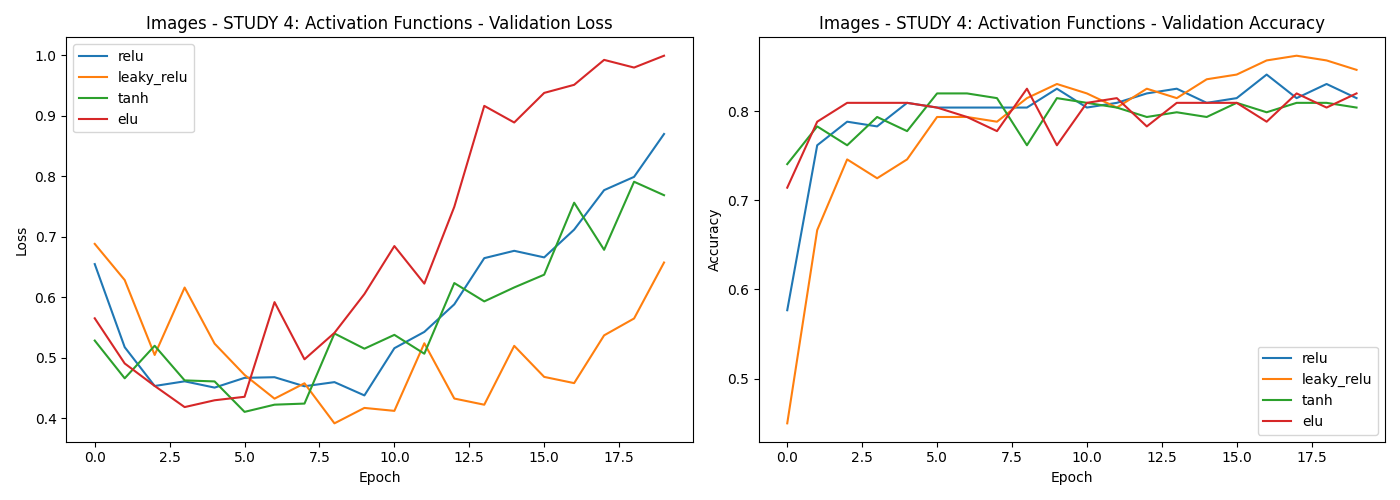
\includegraphics[width=0.9\linewidth]{3Lab/results/activation/img_comparison.png}
    \caption{Aktyvacijos funkcijos tyrimas – vaizdų užduotis}
    \label{fig:rez_aktyvacija_image}
\end{figure}

\begin{figure}[H]
    \centering
    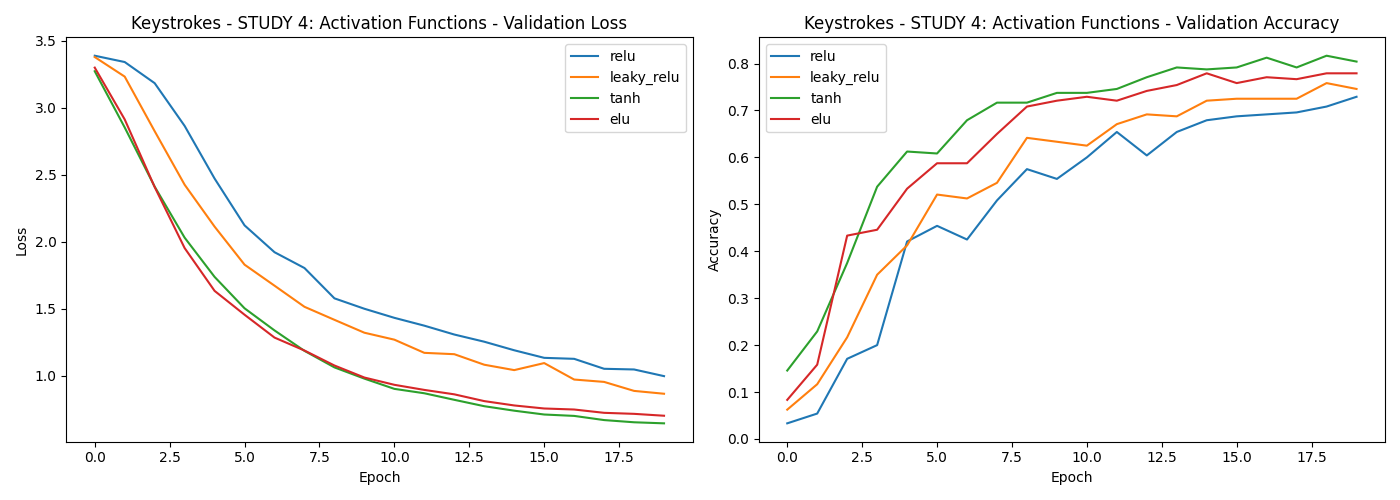
\includegraphics[width=0.9\linewidth]{3Lab/results/activation/ks_comparison.png}
    \caption{Aktyvacijos funkcijos tyrimas – laiko eilučių užduotis}
    \label{fig:rez_aktyvacija_keystroke}
\end{figure}

Pastebimi rezultatai:
\begin{itemize}
    \item Vaizdams visos funkcijos veikia panašiai (\texttt{val\_acc} svyruoja $0{,}82$–$0{,}84$ ribose). Geriausią validavimo tikslumą gavo \textit{ELU}, didžiausią testavimo tikslumą – \textit{LeakyReLU}.
    \item Laiko eilutėms ryškiai išsiskiria \textit{Tanh} – ji geriausiai tinka normalizuotiems $[0,\,1]$ požymiams ($30$ klasių užduotyje pasiekė $\texttt{test\_acc}=0{,}8333$). \textit{ReLU} čia atrodo prasčiausiai – atsineša „mirštančio neurono“ problemą, kai didelė įėjimo verčių dalis yra arti nulio.
\end{itemize}
